\documentclass[11pt]{report}
\usepackage{fullpage}
\usepackage[pdftex,
            pdfauthor={Jeffrey Yoo Warren},
            pdftitle={Grassroots Mapping: a toolkit for participatory and activist cartography},
            pdfsubject={Participatory Cartography},
            pdfkeywords={Cartography},
            pdfproducer={Latex with hyperref},
            pdfcreator={pdflatex,colorlinks}]{hyperref}
\usepackage{graphicx,wrapfig,color,pdfcomment}
\definecolor{linkblue}{rgb}{0.2,0.2,1}
\hypersetup{colorlinks=true,
	    urlcolor=linkblue}

\title{Grassroots Mapping: a toolkit for participatory and politically engaged cartography}
\author{Jeffrey Warren}
\date{May 8, 2010}

%% Define a new 'jeff' style for the package that will use a smaller font.
\makeatletter
\def\url@jeffstyle{%
  \@ifundefined{selectfont}{\def\UrlFont{\sf}}{\def\UrlFont{\small\ttfamily}}}
\makeatother
%% Now actually use the newly defined style.
\urlstyle{jeff}

% Nadya's latex template:
% http://wiki.infosyncratic.nl/LaTeX

\begin{document}
\maketitle

\chapter{Introduction}
\section{Overview}
\section{Defining Grassroots Mapping: Toolkit, Practices, or Community?}

Exactly what makes up the Grassroots Mapping project? Is it a body of code, available under an MIT license at \url{http://github.com/jywarren/cartagen}? Is it a set of mapping practices, or tools, which have been employed in Lima, Peru, or Rio de Janiero? Or is it a community of practitioners and the web site, wiki, and mailing list which tie them together?

Fundamentally this project is intended to make the process of mapmaking easier for lay users, with the intent to broaden participation in cartography. In most places, maps can be seen as a tool of the state and of industry to express control over world we live in. By simplifying the means to create maps, from the data gathering through the editing and publication of digital and print maps, the tools are designed to democratize cartography. In turn, it is hoped that the ability of a broader public to make maps at accessible costs will help to empower bottom-up cartographic activism and to circumvent the current power structure of mapmaking. 

The core of the Grassroots Mapping project is the \textbf{application} of a novel combination of technology to a specific cultural need. Its success, however, is due to the effort and faith of the organizations and individuals who were willing to adopt these new and strange tools, and who saw their potential for use in the communities in Lima, Peru, and the oil spill crisis on the coast of the Gulf of Mexico. This includes Carla del Carpio of Manzanita "A" and Ernesto Fernandez of CEDRO, both in Lima, Peru, and Daniel Miracle and others from Escuelab, also in Lima. It includes Kris Ansin, Shannon Dosemagen, and Anne Rolfes of the Louisiana Bucket Brigade in New Orleans. It also includes the dozens of participants who tirelessly flew kites and balloons, and untangled and wound miles of string day after day.

To make this possible, the project also evolved to include a variety of teaching materials, printed guides, online videos, and workshops, both by the author and by the diverse collaborators who took ownership of the tools. These materials spanned a broad range of audiences, from 10-15 year old Spanish-speaking students to environmental activists in West Virginia and Kentucky. 

Ultimately, even the digital tools, including the Cartagen map rendering framework and the Cartagen Knitter, a tool for orthorectifying aerial imagery, were built with assistance and support of UROPs, colleagues, and contributors in the broader mapping community. That this has become the norm in technology projects does not detract from the fact that much of this work would have been impossible without such contributions. 

Building tools is unlike developing more abstract technologies in that to be successful, a series of compromises and pragmatic decisions must guide the design process, as well as continuous communication with an audience of users. The Grassroots Mapping project has evolved inresponse to these needs and should be examined in the context of the specific uses it has attempted to address, rather as an isolated or 'pure' work.

\subsection{Audience and process}

The tools developed as part of the Grassroots Mapping project address the needs of both committed enthusiasts who need powerful and efficient mapping technology, as well as those who have little experience and expertise but need simple and direct tools to make maps. Therefore, some of the tools, while being simple to use, are intended for 'power users' or those technically fluent in writing and editing code. The Cartagen framework falls under this category. Other tools, such as the balloon- and kite-based platforms for capturing aerial imagery, are intended for a wider audience, as is the Cartagen Knitter, a specific use of the Cartagen framework. A description of the various tools follows.

\subsection{Software}

\subsubsection{Interfaces for participatory cartography}

This section focuses on the framing, intent, and audience of the tools. A technical discussion of the tools can be found in Chapter 8. 

\subsubsection{The Cartagen framework}
\subsubsection*{Rendering architecture}
\subsection{Hardware}
\subsubsection{Balloon Aerial Photography}
\subsubsection{Photography from Kites and Unmanned Aerial Vehicles}
\subsection{Practice, Community, Support structure}
\subsubsection{GrassrootsMapping.org}
\subsubsection*{The Grassroots Mapping Wiki}
\begin{wrapfigure}{r}{0.5\textwidth}
	\begin{flushright}
		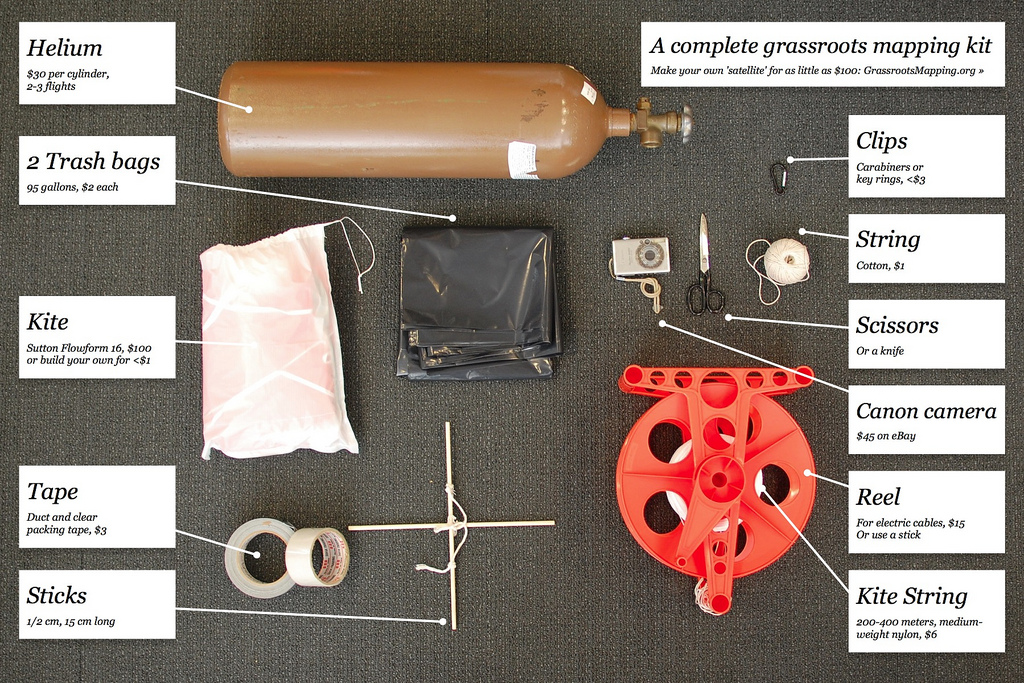
\includegraphics[width=0.45\textwidth]{images/100-dollar-satellite-poster.jpg}
	\end{flushright}
\end{wrapfigure}

\subsubsection*{Printed guides and support materials}
\subsubsection*{Curricular guides and teaching notes}

\subsubsection*{Documentation, case studies, Grassroots Map Collection}
\subsubsection*{The Grassroots Mapping community and mailing list}
\section{Novel Contributions}
\subsection{Novel application of low-cost tools to well-established need for raster imagery}
%\pdfcomment{do we discuss existing systems here? no, just mention paradigms of tiles, reference later section}

\subsection{Novel approaches to map rendering}
\subsection{Central merit: technology or culture?}
%both, duh: technology is only relevant in a context, and I make no attempt to separate this technology from its intended sociopolitical meaning

\chapter{Subjectivity in Mapping}

% text here, why is this chapter necessary:

The need for a more participatory cartography is predicated on the exclusion of many from the practice of map-making as it stands today. Even more importantly, it depends on the point of view that mapping is an inherently non-neutral practice, and that for maps to serve wider and more democratic interests, it must accommodate diverse viewpoints. Maps serve interests, and understanding their role not as documentation of what makes up the world, but as rhetorical, tactical, and \emph{subjective} tools is an important prerequisite to what this document argues.

\section{Neogeographers, Psychogeographers, and GIS}

A brief description of three distinct groups of practitioners is worthwhile, as each embodies a distinct conception of mapmaking. 

\subsection{Psychogeography}

\subsection{GIS practitioners}

Professional map makers have used Geographic Information Systems, or GIS since its development in the 

\subsection{Neogeography}

With the rise of web-based data and display systems came a group composed primarily of programmers and web designers, who have adopted the name \emph{neogeographers}. This group positions itself in contrast to 'traditional' approaches such as GIS, and 

% ... incomplete

Rana and Joliveau suggest that neogeography rejects the 'prescribed role/interaction between the four main components, namely the audience, the information, the presenter and the subject...'. 

% rana-joliveau-neogeography.pdf, 'NeoGeography: an extension of mainstream geography for everyone made by everyone?

% ... incomplete

Andrew Turner: Introduction to Neogeography
coined by Di-Ann Eisnor?
http://apb.directionsmag.com/archives/1379-Define-Neogeography.html

"outsiders"

\url{http://books.google.com/books?id=oHgDv4feV-8C&dq=neogeography+turner&printsec=frontcover&source=bn&hl=en&ei=gmDLS6_-KYj98AaY_KWXDA&sa=X&oi=book_result&ct=result&resnum=5&ved=0CBwQ6AEwBA#v=onepage&q&f=false}

"NeoGeography and the nature of geographic expertise", Author: Michael Goodchild  \url{http://www.informaworld.com/smpp/content~db=all~content=a911734343}
% goodchild-michael-neogeography.pdf

Orig. ref to Platial's usage: \url{http://placekraft.blogspot.com/2006/04/neogeography-defined.html}

% NEED reference for start of GIS practices 

\section{The mythical 'complete' map}

The most famous (yet fictional) version of this fantasy is Jorge Luis Borges' short story 

'a mile to the mile!'
'So we now use the country itself, as its own map, and I assure you it does nearly as well.' p.169

This idea was later elaborated in Jorge Luis Borges' 

% Of Exactitude in Science

% ...In that Empire, the craft of Cartography attained such Perfection that the Map of a Single province covered the space of an entire City, and the Map of the Empire itself an entire Province. In the course of Time, these Extensive maps were found somehow wanting, and so the College of Cartographers evolved a Map of the Empire that was of the same Scale as the Empire and that coincided with it point for point. Less attentive to the Study of Cartography, succeeding Generations came to judge a map of such Magnitude cumbersome, and, not without Irreverence, they abandoned it to the Rigours of sun and Rain. In the western Deserts, tattered Fragments of the Map are still to be found, Sheltering an occasional Beast or beggar; in the whole Nation, no other relic is left of the Discipline of Geography.

% From Travels of Praiseworthy Men (1658) by J. A. Suarez Miranda

% The piece was written by Jorge Luis Borges and Adolfo Bioy Casares. English translation quoted from J. L. Borges, A Universal History of Infamy, Penguin Books, London, 1975.

The idea that maps accurately, or even completely depict a location is not entertained in a literal sense, yet amongst

% Title: UK Motorways 100% Complete
% I'm pleased to announce that the main carriageways of all mainland UK motorways have been completed.  Over 3,000 km of roadway.
% Etienne Cherdlu Sat Jan 7 10:45:05 UTC 2006

\begin{wrapfigure}{r}{0.5\textwidth}
	\begin{flushright}
		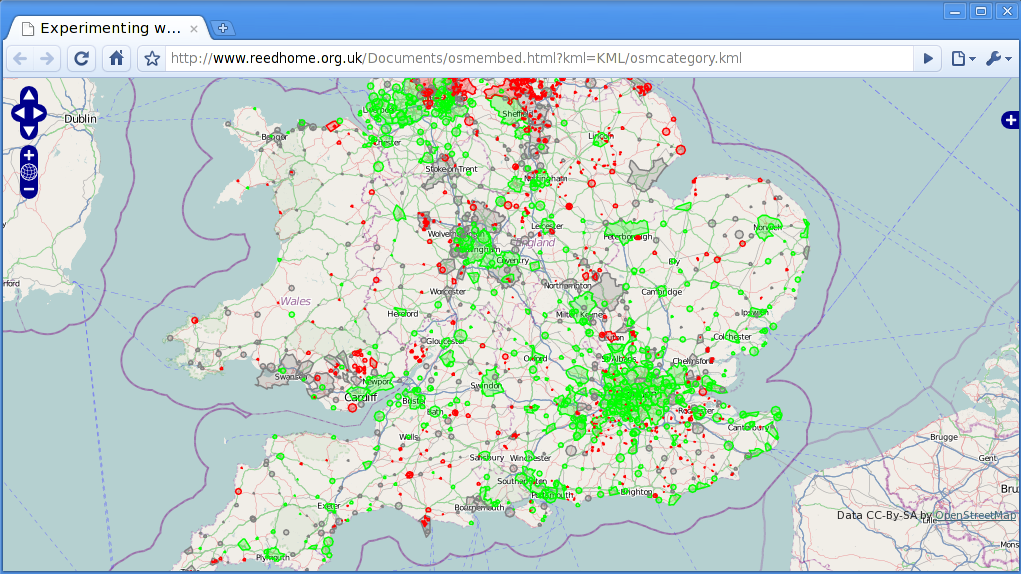
\includegraphics[width=0.45\textwidth]{images/osm-missing-parts.png}
	\url{http://www.reedhome.org.uk/Documents/osmembed.html?kml=KML/osmcategory.kml}
	\end{flushright}
\end{wrapfigure}

Chris Anderson 

%We often imagine 'complete maps'
% Epistomology and mapping: maps are a form of technology, and of power      
%  - OSM reference to a 'complete map of UK'
%        - Chris Anderson's Wired article of complete dataset
% "At the petabyte scale, information is not a matter of simple three- and four-dimensional taxonomy and order but of dimensionally agnostic statistics. It calls for an entirely different approach, one that requires us to lose the tether of data as something that can be visualized in its totality. It forces us to view data mathematically first and establish a context for it later."
% Read More http://www.wired.com/science/discoveries/magazine/16-07/pb_theory#ixzz0lTiRSTXp
% rebuttal: http://www.edge.org/documents/archive/edge248.html#hillis
\section{Maps as a 'window' onto the world}

% essentially epistemological issue.

For a variety of reasons, maps carry the weight of authority in a way that few other forms of evidence do; the main driver being the widely held belief that satellite or aerial maps are a kind of 'window' into the world. In photography the editorial role of the author is accepted, not to mention the damage which 'photoshopping' has inflicted on the perceived truth or even objectivity of the photographic image. Maps, however, continue to be taken as direct representations of reality, desipte the inherent subjectivity of image selection, color, brightness, and contrast processing, and the editorial eye necessary in reading and interpreting such imagery. 

\begin{wrapfigure}{r}{0.5\textwidth}
	\begin{flushright}
		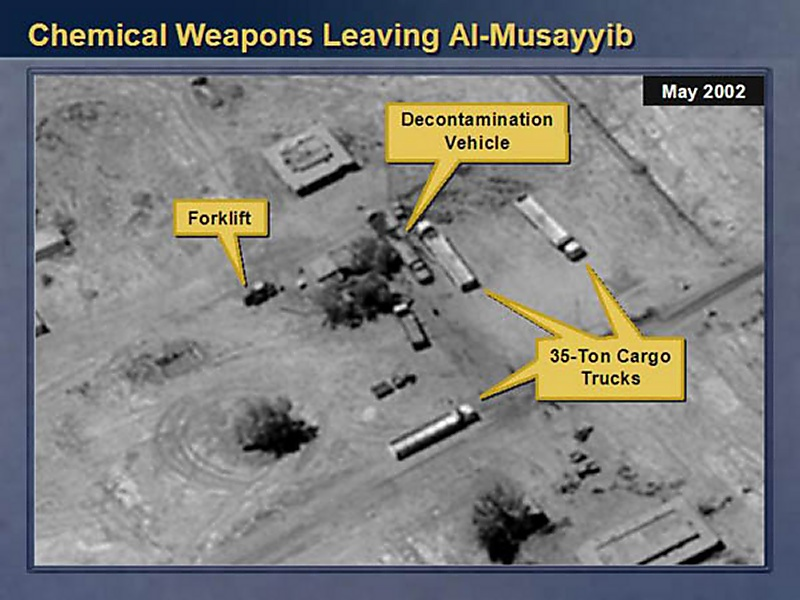
\includegraphics[width=0.45\textwidth]{images/February_5,_2003_trucks_at_the_Al_Mussayyib_chemical_complex_along_with_a_decontamination_vehicle.jpg}
	\url{http://en.wikipedia.org/wiki/File:February_5,_2003_trucks_at_the_Al_Mussayyib_chemical_complex_along_with_a_decontamination_vehicle.jpg}
	
	\end{flushright}
\end{wrapfigure}

The best example of this attitude is of course the use of relatively low resolution satellite imagery by Colin Powell at the UN Security Council in February 2003, used as evidence to support the existence of weapons of mass destruction in Iraq. The subsequent complete absence of weapons did little to diminish the public's faith in such imagery as objective evidence. 
% citation http://www.un.org/apps/news/storyAr.asp?NewsID=6079&Cr=iraq&Cr1=inspect 
% Fallacy!!! Wood, p. 20,21 - centimeter accuracy gives false impression of 'scientific accuracy' and completeness

What is most alarming about this kind of rhetorical use of map imagery is that it represents a means for those in a position of power to assert truths about places they have never been, without the involvement of human testimony from those who have.

This aspect of the public perception of maps as an objective, quantitative measure may have a relationship with the difficulty and expense of producing map imagery, and the traditional monopoly of government and high-tech industry in the production of such imagery.

\section{Maps: rhetorical, even tactical}
%        - Endless variety of possible data: Wood, Power of Maps, p.1
%        - not a representation of truth, but a rhetorical tool; Wood, p1?
%            - social construction of maps
% 	- map of sewer system from Wood
%	- Tactical cartography from Institute for Applied Autonomy
%	- http://www.tacticaltech.org/mapsforadvocacy
\section{Ground Truth, or maps as testimony}
%    - varying definitions of ownership, contested terrain
%        - 'Ground Truth' policy in OSM (http://wiki.openstreetmap.org/wiki/Disputes#On_the_Ground_Rule)

\section{Cartographic ethics}

Cartography, ethics, and social theory: \url{https://commerce.metapress.com/content/c21115120603xj14/resource-secured/?target=fulltext.pdf&sid=gb5vtk2lhvt0dj55c1xba4aa&sh=utpjournals.metapress.com}

% THIS WHOLE SECTION SHOULD PERHAPS BE MOVED TO 'DISCUSSION', post-Peru, or just after introducing state of the art... it may be a whole chapter.

PGIS: 
Do your best to recognise that you are working with socially differentiated communities and that your presence will not be politically neutral
Be considerate in taking people’s time
(bibliography/rambaldi-practical-ethics-for-pgis.pdf)

Chambers, chambers-who-empowered-disempowered-gains-loses.pdf
Outline of history and benefits of PGIS, but also of ethics and beneficiaries

\subsection{Subjective cartography in practice}
%    - ref. West Bank mapping in Dec 2009
% Tree symbolism
% B'Tselem map of settlements
%        - mapping as testimony of use/presence/ownership by Abed's farm

\chapter{The Need for Geospatial Data}
\section{Two worlds of mapping}
\subsection{Urban slums, informal settlements}
%    UN-HABITAT quotation
%	- “geographical mapping techniques to support struggles for social justice in India”. The end result, it added, could make maps as “tools to fight injustice in society”.
%	- http://timeoutbengaluru.net/aroundtown/aroundtown_feature_details.asp?code=59

Brief outline of fulfilled needs: chambers-who-empowered-disempowered-gains-loses.pdf, p.4

\subsection{Tenure mapping}
\subsubsection{The invasion of Lima, Peru}
%        - El Otro Sendero
%            - graph of informal settlement percentages
%        - COFOPRI

\subsection{Mapping: a tool of empowerment or control?}

Evgeny Morozov, "How dictators watch us on the web" - \url{http://www.prospectmagazine.co.uk/2009/11/how-dictators-watch-us-on-the-web/}
\url{http://irevolution.wordpress.com/2010/01/07/morozov-vs-shirky/} (Patrick Meier)

many criticisms may represent limited experience mapping... circular?
It is easy for activist cartographers who do not live in a community to advocate the use of tools which may put that community at risk.

"empowerment":(great article on definitions for empowerment and framework for discussing empowerment in the PGIS context)

Corbett, Jon M., and C. Peter Keller. 2005. An Analytical Framework to Examine Empowerment Associated with Participatory Geographic Information Systems (PGIS). Cartographica 40 (4):91-102.

\section{Environmental assessment}
\subsection{Asset allocation mapping and carbon cowboys}

%	- bibliography/poole-peter.pdf
%	- stewardship of biodiversity, p.2
%	- case study uses of mapping capability, p.5
%	- detecting and monitoring impacts of industrial-scale development

\section{Open geodata and crisis mapping}
\subsection{Crisis mapping and Ushahidi}
%	- origin in political mapping, focus on natural disaster
%        - UN-SPIDER/Google MapMaker response to Mikel Maron, Chile Earthquake

\chapter{State of the Art}
\section{PGIS: Participatory Geographic Information Systems}

Traditional GIS technology has been used since the XX's to support communities in developing contexts for purposes such as making tenure claims, environmental defense against petroleum and other extraction industries, as well as for planning purposes. This has become known as PGIS, or Participatory GIS, and typically... 

% See Peter Poole's Life after Tenure Mapping for a brief historical timeline, i think

\subsection{PPGIS}

Definition: \url{http://www.ppgis.net/ppgis.htm}
Bibliography: \url{http://dusk2.geo.orst.edu/gis/student_bibs/slurie.htm}


bibliography/rambaldi-participatory-spatial-developing-countries.pdf

\subsection{Participatory GIS for Development}
% Jen Osha's article
%\href{http://www.directionsmag.com/article.php?article_id=2365&trv=1.}{Participatory GIS - A Paradigm Shift in Development?} - Jen Osha and Daniel Weiner, 2006
%        THE ILLUSTRATED GUIDE TO NONPROFIT GIS AND ONLINE MAPPING: http://maptogether.org/nonprofit-mapping
%        Claudia Canepa's PhD dissertation
\subsection{Shortcomings of traditional PGIS practice}
%    Peter Poole - Life after Tenure Mapping
%        - outsourcing of GIS processing typical, problems
\section{OpenStreetMap}

% OSM acronym

\subsection{Humanitarian OSM Team}
%   HOT acronym
\subsubsection{Free Map Gaza}
%        Map Kibera, Free Map Palestine, Free Map India
\subsubsection{Followup projects}
%        Data modeling: http://wiki.openstreetmap.org/wiki/Humanitarian_OSM_Tags/Humanitarian_Data_Model
\subsubsection{Challenges}
%        Slum mapping, disaster-specific issues
%        architectural/infrastructural shortcomings
%	reliance on GPS, or need for a base layer
% 	inclusion in a GPS-device process
%	ease of use, black-boxing of information
%	JOSM, other issues with typical deployment
\textbf{Emphasis on local infrastructure}

\chapter{Grassroots Mapping as an alternative means of participatory cartography}
%    Meet subjectivity needs
%        - against a canonical datastore
%        - solution lays in tools and formats and practices, not in a single project/datastore
%            - therefore GM & Cartagen are based around:
%                - a body of code
%                - a thorough documentation and guide to mapping techniques
%        - options to organize project: as a 'generic hub' for imagery, like OpenAerialMap, engage primarily via internet/blogs
%            - or, focus on collaborating with specific communities in cartographic dispute
%                - expand into matchmaking between mappers and communities in need, as well as supporting via mailing list 
%                - maintain open communication with end-users, iterate back into tools: 
%                    - requests made via list: stewart long asks for masking, Crispen asks for entry of lat/lon pairs, WhereCamp folks asked for locking, Pat Coyle asked for 'natural_size' feature
\section{Cartagen: an alternative architecture}
%        - existing solutions based around cloud systems
%            - this move opposite - closer to client
%            - needs: data under no connectivity
%            - multiple devices
%            - ownership of data/infrastructure
%                - FrontlineSMS, 'local' is a feature, opposite of corporate/commercial strategy
%        - low-AI approach; technical literacy, flexibility, admits 'misuse'
%            - examples: USGS overlay at WhereCamp 2010
%            - additon of non-map features with Warper tool
%            - difficulty of use of hugin, etc
%                - DIYDrones thread: "3 days stitching and tweaking images" (http://diydrones.com/profiles/blog/show?id=705844:BlogPost:134855&page=1#comments)
%            - Stewart Long uses Photoshop for most stitches (get him on record)
%Emphasis on building in response to end-user needs
%    - this work could only be done by working with communities in cartographic dispute. See Lima case study.

\chapter{Related works}
%    Inspiration, context, history of activist/grassroots mapping
%    Reiterate HOT/Free Map Palestine, India, Kibera
%    GroundTruth, Jai Sen, A People's Atlas of Chicago
\section{Beyond symbolic mapping: Data-driven approaches to participatory mapping}
%        Expanding role of mapping to legal, tactical
%        Institute for Applied Autonomy

\chapter{Evaluation criteria}
\section{Participants vs. collaborators}
%        Role of Carla, Escuelab, Shuawa
%        Hector as a fellow educator (interview)
%    'Reconceptualizing Validity' (Patti Lather, p.67)
\subsubsection{Triangulation}
\subsubsection{Construct validity}
how theory was affected by data
\subsubsection{Face validity}
how research was received by participants
\subsubsection{Catalytic Validity}
how participation transforms the situation (self-awareness/reflexivity)

\subsection{Interviews with local partners}
Wiki, mailing list, blog, media coverage (~ Face validity)

\chapter{The Grassroots Mapping tool chain}
\section{Balloon/kite Aerial Mapping (BAM/KAM)}
%    UAV - DIYDrones and collaboration (see 'Future work')
%        Leveraging both expert and 'amateur'/enthusiast expertise
%        Connecting hobby/DIY communities with activist communities and agendas
\subsection{Accuracy and precision in kite and balloon imaging}
% focus on cost goals, 'mapping at all'
% Eric Wolf's thesis on BAP metrics: wolf-eric-thesis.pdf

\section{Digital maps: reconceptualizing mapping interaction}
\subsection{Beyond raster mapping/Tile politics}
%            Metadata: authorship data
%            Google Maps png metadata hack
%            GIS and broadly adopted consumer-focused mapping stacks
\subsection{Cartagen dynamic rendering}
%            Existing vector systems (Chris Schmitt's email on geowanking)
%            Limitations: technical, barrier-to-entry, participatory, literacy
%                GSS (and OSM-JSON): appropriating the HTML/CSS paradigm for data legibility and open access
%                    Format politics: XML, JSON, RSS
\subsection{An iterative toolchain development process}
%    Toolchain not developed in vacuum, but through collaboration and study on-site
%        - initial flight testing with Josh Levinger
%            - MIT map
%            - terrain, difficulty
%            - optimization for site: Peru, low buildings, no trees
%        - Peru, West Bank, India
%        - Following chapters document those collaborations and their fruits

\chapter{Case Study: Grassroots Mapping in Lima, Peru}

\section{Introduction}

In the interest of basing tool development and design on real-world applications, and due to an ongoing conversation with Carla del Carpio of Lima-based Manzanita "A", 

traveled to Lima, Peru in January 2010 to conduct field research and to collaborate on the Grassroots Mapping tool set with those who would be likely to use it.

\subsection{Designing with, not for}

Needs assessment

Potential beneficiaries/collborators: Hector, Carla/Manzanita A, CEDRO, Escuelab, Shuawa

\subsection{The Other Path: Lima's history of informal settlement}

%    Suitability of Peru - history of 'invasions'
%        - de Soto's work; tenure 9x value

\subsection{Valuation and 'grey' economies}

%        - asset mapping; NiJeL, informal economies

\subsection{Limits of state-sanctioned mapping efforts}

%        - COFOPRI and history of ineffective state-led mapping/legalization processes
%    Current approaches to mapping: 
%        COFOPRI, engineering firms, comparisons with OSM-HOT, UN-SPIDER from earlier discussion

\subsection{A Grassroots Mapping curriculum}

%    Development as a curriculum
%        Importance of understand political/social role of cartography

\subsection{Mapping with Juan Pablo II}

%            - CEDRO & Manzanita "A"
%            - size, ages, of kids
%            - outline of activities
%                - (Illustration of timeline)
                - Introduction to mapping
                    - discussion: literal mapping difficult due to different mental models
                    - tape-measure technique -- bodystorming
                    - introduction to Google imagery not relevant
\subsubsection{First flights in Juan Pablo II}

%                - Initial balloon flights
%                    - technical issues
%                    - difficulty in involving kids in process
%                        - note: thought about potential for each student to build a satellite: want to try
%                    - immediate interest & success amongst community members

\subsubsection{Situating mapping practice}

%                - Printing & review of images
%                    - unanticipated interest in seeing selves from above
%                - History & Future exercises
%                    - Having seen community from above made representation easier
%                    - interspersed with flights
%                    - very specific information about construction/infrastructure from Frank & others
%                    - maquette in 3D - unsolicited - wealth of specific information about goals
%                        - 3 story buildings (sendero - stored wealth/bank accounts)
%                        - explicit connection between mapping and urban planning
%                        - real engaging activity as a corollary to mapmaking
%                        - references to infant care (WaWaWasi), shops, flowers, soccer fields
%                        - Project Morrinho maquettes in Brazil

\subsubsection{Stitching maps with Juan Pablo II}
                - Stitching exercises
                    - with kids - 'rubber sheets'
                        - with teachers (secondary audience) - Map Warper, discussion of difficulties (see ahead)

\subsection{Mapping with San Ignacio Loyola}
% (have title and survey)
            - Manzanita "A"
            - usage of Photoshop primarily; fast mapping; 2-3 hrs flight, 1-2 hrs stitching
            - Hector: ideal user: 
                - lives in an informal settlement
                - teacher, interested in using this in curriculum
                - community leader
                - interest in tech, willing to try map warping
                    - difficulty in trackpad/menu usage, took notes
                - engaged despite workload
                - sees applicability for mapping tools in settlements

\subsection{Mapping with Cantagallo}
            - Escuelab - technology, art, society
            - engaged with a creative group, Shuawa
\subsubsection{The Shipibo in Lima}
            - narrative of 10 year stay, claim to land, contested claims, and riverbank site
            - Escuelab sought political neutrality, but obviously interested in political situations: ex: shipibo language            - Drawing exercises
                - 'amazon' home vs current home
                - non-literal mapping - related to issues of veracity re: Wherecamp sugg. of children mapping with stickers
\subsubsection{Flying balloons with Cantagallo}
- fastest yet
                - total images
                - usage of hugin/SIFT/Photoshop
\subsubsection{Lower Cantagallo and local geographic dispute}
            - Escuelab and Sara/CEDRO
	- two cantagallos (three?)
            - Sr. Ricardo - possible political engagement/entanglement
            - entry into SETAME site; playfulness seen as neutrality? Or just no resistance at low levels to mapping activity?
                - not perceived as claim-related?
\subsection{Computing literacy challenges with orthorectification}
	- map warper
        - designed for printed maps
        - large loop of interaction - overcorrection easy, no immediate feedback upon assigning GCPs
        - difficulty in explaining GCPs, and necessity of javascript hack for areas without base data
        - amazing for intended use, even note application in Mumbai
    - Photoshop better, but barely
	- stuart long uses photoshop, maybe bruce owen (see emails)
\subsection{Evaluation}
- based on criteria
        - Interviews!!!!!!! transcribe them
        - Applications of maps we made
            - legal role
            - import to OSM?
            - World Bank mandate to map every home? do we support that goal?
            - education, urban planning, NGO planning support, demonstration project
\subsection{Needs (Re)assessment}
- Goals for a true 'pilot' that goes beyond information gathering and use of existing State of the art tools
   - planning of new, easier interfaces and techniques
                - Map Warper difficulties, speed
            - discussion and 'designing with' leading to Cartagen Knitter (see later discussion)
		- http://en.wikipedia.org/wiki/Rubbersheeting
            - needs assessment - user-centric design, appropriate design
    - Possibility of mapping a fast-changing community
        History/future assignments make explicit the value of mapping as an activity

\chapter{Citizen mapping of the BP oil spill}
\section{Grassroots mapping in crisis response}

In late April 2010, the Deepwater Horizon oil rig exploded and sank, initiating what may be one of the worst environmental disasters in US history. As the spill grew in size, the author contacted Stewart Long of GonzoEarth.org and Oliver Yeh of 1337arts.com. Long has used remote control aircraft to produce maps, and Yeh specializes in high-altitude photography using weather balloons, having captured imagery from a balloon at altitudes of over 90,000 feet. The three decided to travel to the Gulf Coast area to spearhead a citizen effort to map the oil spill's effects. After making phone contact with Anne Rolfes of the Louisiana Bucket Brigade (LABB), a New Orleans-based environmental activist group, Yeh and the author flew to New Orleans on May 5th 2010, followed by Long on May 6th. 
% env. crisis in US history: http://www.npr.org/templates/story/story.php?storyId=126410895
% http://www.nytimes.com/2010/04/25/us/25rig.html - Oil Leaking Underwater From Well in Rig Blast, By CAMPBELL ROBERTSON, April 24, 2010

With the cooperation and extensive support of the LABB and other interested New Orleans residents, the team began leading almost daily trips to use balloons and kites to map coastal areas. While not attempting to produce imagery of the entire at-risk coastline, which stretches several thousand miles from Louisiana to Florida, the mappers focused on acquiring high resolution imagery of specific sites, with the goal of producing 'before and after' maps. The trips relied on the availability of free transport to affected areas, but in the initial days of the project this was not a problem, as fishermen and charter companies began calling in to offer their services for free. Increasingly large areas of the Gulf of Mexico were being closed to fishing, and with their livelihoods at risk, many in the fishing industry were eager to participate in the documentation of the spill. 

% fishery closings: http://sero.nmfs.noaa.gov/deepwater_horizon_oil_spill.htm 

The 2010 Gulf oil spill was seen as an opportunity to apply the low-cost mapping techniques refined and documented on GrassrootsMapping.org to a problem of immediate import. While many overflights were occurring, there was no publicly available, orthorectified imagery available in the initial weeks of the spill; up-to-date imagery was supplied mainly by the MODIS (Moderate Resolution Imaging Spectroradiometer) sensors aboard NASA's Terra and Aqua satellites. MODIS is limited to 1000 meter resolution for those bands which are used for ocean imaging, and while the daily images available were very useful in determining where along the coast was being hit by slicks and sheens, it was not of high enough detail to show any specific damage. 

% http://modis.gsfc.nasa.gov/about/specifications.php

By contrast, the imagery collected by the LABB/Grassroots Mapping teams was up to 5 cm/px in resolution, and could be repeatedly captured over the course of days or weeks.  


\chapter{Field trials in India}
\section{Goals}

\chapter{Project sustainability and ongoing work}
\section{Wiki, blog and mailing list}
        Incorporation of new needs through dialogue (see Evaluation Criteria .. Face validity/Construct validity)
        Examples of community-based reformulation/innovation
            Crispen's suggestion of lat/lon rectification points (mentioned above)
            Pat Coyle's videos, bungee-cable design, and camera shutdown research

\section{Illustrated Guide}
        Nathan Cooke, Pat Coyle
    Workshops/flights
    Community building, matchmaking (mentioned in strategies section above)



\begin{figure}[h]
  \begin{center}
    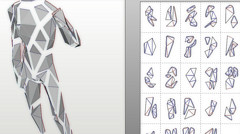
\includegraphics[scale=0.75]{images/test.jpg}
    \caption{The Toucan}
  \end{center}
\end{figure}

\chapter{ReadingList}

\hypertarget{related_readings_1}{}\subsection*{{Related readings}}\label{related_readings_1}

A collection of readings on kids, playful exploration, and grassroots mapping

\textbf{Jeff:}

\href{http://dspace.mit.edu/handle/1721.1/33012}{New information technologies in the old political economy : an exploration of community-based GIS for improving basic services for the poor in New Delhi, India} - 2005 MIT DUSP dissertation by Claudia Canepa

\href{http://www.ejisdc.org/ojs2/index.php/ejisdc/article/viewFile/237/158}{PARTICIPATORY SPATIAL INFORMATION MANAGEMENT AND COMMUNICATION IN DEVELOPING COUNTRIES} - Giacomo Rambaldi, Peter A Kwaku Kyem, Mike $\backslash$McCall, Daniel Weiner, EJISDC, 2006

\href{http://books.google.com/books?id=4u79ffyzekoC&printsec=frontcover&dq=child%27s+pictorial+world&ei=5EUYS9veGqPqygShs7TVBw#v=onepage&q=&f=false}{The child'{}s creation of a pictorial world}, Claire Golomb

\href{http://www.unicef.org/teachers/researchers/intro.htm}{Curriculum on ``{}Children as Community Researchers''{}} - UNICEF, authored by \href{http://web.gc.cuny.edu/che/cerg/about_cerg/environmental_learning_index.htm}{Children'{}s Environment Research Group}

\href{http://www.directionsmag.com/article.php?article_id=2365&trv=1.}{Participatory GIS - A Paradigm Shift in Development?} - Jen Osha and Daniel Weiner, 2006

\href{http://www.iapad.org/pgis2005/}{Mapping for Change} - 2005 International Conference on Participatory Spatial Information Management and Communication

Weiner, D. and T. Harris, 2003. ''{}\href{http://www.rri.wvu.edu/pdffiles/gisweiner.pdf}{Community-Integrated GIS for Land Reform in South Africa}.''{} URISA Journal. 15(2): 61-73.

\href{http://www.maptogether.net/taxonomy/term/151}{PPGIS on MapTogether.net}

\href{http://books.google.com/books?hl=en&lr=&id=_VK-ABCKlVgC&oi=fnd&pg=PA3&dq=Nino+Bariola&ots=_r1wMwjiou&sig=TH0Gn1P27Xtsdq2Oc0Up5D6HLzg#v=onepage&q=Nino%20Bariola&f=false}{Bilingualism and identity: Spanish at the crossroads with other languages} - Geographic dispute in Canta Gallo, in Lima, \href{http://books.google.com/books?id=_VK-ABCKlVgC&lpg=PA3&ots=_r1wMwjiou&dq=Nino%20Bariola&lr=&pg=PA153#v=onepage&q=&f=true}{Chapter 7}

\href{http://www.sciencedirect.com/science?_ob=ArticleURL&_udi=B6VG2-4XHJX4B-1&_user=10&_coverDate=08/31/2009&_rdoc=1&_fmt=high&_orig=search&_sort=d&_docanchor=&view=c&_searchStrId=1186930669&_rerunOrigin=google&_acct=C000050221&_version=1&_urlVersion=0&_userid=10&md5=a9327ffa62e089e863f892a4551c1717}{Intervention: Mapping is critical!} - This intervention targets the much heralded demise of the map in geography and the recently proposed “rethinking” of maps. It comprises contributions from two political geographers, a military geographer, a political scientist, and two activist cartographers and argues that there is not so much a need to “rethink” maps, but to “re-engage” with the material practices of mapping, and above all to “re-make” maps.

\href{http://training.esri.com/campus/library/bibliography/RecordDetail.cfm?ID=95545&browseonly=0}{Mapping in a Shoebox} - A Grassroots Approach for Developing the Geospatial Literacy of Elementary Children - 24th International Cartographic Conference - Jaqueline M. Anderson, Sally Hermansen, Lorraine Innes, 2009

Lots of work by Proboscis: \href{http://urbantapestries.net/}{Social Tapestries/Urban Tapestries}, 2002-7 - Urban Tapestries investigated how, by combining mobile and internet technologies with geographic information systems, people could `{}author'{} the environment around them; a kind of Mass Observation for the 21st Century. Like the founders of Mass Observation in the 1930s, we were interested creating opportunities for an ``{}anthropology of ourselves''{} – adopting and adapting new and emerging technologies for creating and sharing everyday knowledge and experience; building up organic, collective memories that trace and embellish different kinds of relationships across places, time and communities.

\href{http://www.geoconnections.org/publications/Key_documents/Sensitive_Env_Geo_Data_Guide_EN_v1.pdf}{BEST PRACTICES FOR SHARING SENSITIVE ENVIRONMENTAL GEOSPATIAL DATA} - for GeoConnections by AMEC Earth \& Environmental, 2010

\textbf{Kate:}

\href{http://news.bbc.co.uk/2/hi/uk_news/8216071.stm}{BBC article} - train station hires a Director of Fun!

\href{http://www.rajworks.com/index1.htm}{Place-Logging} - MIT thesis

\href{http://www.youtube.com/watch?v=U2uH-jrsSxs&feature=rec-LGOUT-exp_fresh+div-1r-3-HM}{Tube iphone app} - augmented reality

\end{document}
